\section{Introduction}
\label{sec:intro}

The exponential growth in deep neural network parameters and dataset scales has made multi-task training from scratch computationally prohibitive. To address this, parameter-space \emph{model merging} has emerged as an elegant and resource-efficient paradigm for multi-task learning \citep{ilharco2022editing, wortsman2022model}. Rather than performing expensive multi-task fine-tuning, model merging aggregates the weights of multiple task-specific expert models, each independently fine-tuned from a shared pre-trained base model $\theta_0$. Foundational techniques such as Task Arithmetic \citep{ilharco2022editing}, TIES-Merging \citep{yadav2023ties}, and DARE \citep{yu2023language} utilize direct linear or sparsified addition of task-specific weight differences (task vectors).

Despite their empirical utility, static merging methods rely on uniform scaling coefficients across all layers, ignoring the highly specialized and depth-dependent hierarchical representations within deep neural networks. To overcome this limitation, \citet{adamerging} proposed \emph{AdaMerging}, a framework for adaptive model merging. AdaMerging introduces learnable layer-wise merging coefficients $\boldsymbol{\lambda} \in \mathbb{R}^{K \times L}$ and optimizes them online during test-time adaptation (TTA) using gradient-based minimization of the Shannon entropy of predicted probability distributions \citep{wang2020tent, liao2021are}. 

However, we argue from a theoretical perspective that unconstrained optimization in deep neural network parameter spaces is fundamentally ill-posed and mathematically hazardous. During test-time adaptation, the model must adapt to a local, unlabeled stream of incoming test data, which is frequently subject to transductive bias and noise. When the layer-wise merging coefficients $\boldsymbol{\lambda}$ are allowed to optimize without constraint, the optimizer minimizes prediction entropy by overfitting to this local transductive stream. It does so by generating high-frequency spatial oscillations in adjacent layer coefficients, effectively routing representation features through disjointed scales across the network depth. Under the physical laws of representation learning, such uncoordinated, high-frequency oscillations disrupt the internal representation manifold of the transformer, leading to a catastrophic collapse of features and a severe drop in generalization performance. 

We formalize this critical failure as the \textbf{Overfitting-Optimizer Paradox}: \emph{unsupervised local optimization of merging coefficients fits transductive noise, resulting in degenerate representation collapse and worse multi-task generalization than static uniform baselines.}

To resolve this paradox, we propose that the optimization of merging coefficients must be bounded by the intrinsic second-order geometry of the pre-trained loss landscape. We model the parameter space of the deep network not as a flat, isotropic Euclidean surface, but as a \emph{Riemannian manifold}, where the distance between parameter configurations is locally scaled by the curvature of the loss function. Our framework, \textbf{Riemannian Curvature-Regularized Test-Time Model Merging (RCR-Merge)}, implements this geometric philosophy. 

Specifically, we pre-compute the trace of the diagonal Fisher Information Matrix (FIM) for each layer of the base model on a minuscule calibration set, which serves as a highly localized metric of parameter sensitivity (curvature). During test-time adaptation, we apply a novel spatial regularizer, \emph{Riemannian Curvature-Weighted Total Variation (RCR-TV)}. This regularizer penalizes the squared difference of merging coefficients between adjacent layers, scaling the penalty dynamically by the geometric mean of their pre-trained base curvatures. 

By grounding the spatial regularizer in physical base curvatures, RCR-Merge creates an analytical barrier: in highly sensitive bottleneck regions of the loss landscape, any sudden, high-frequency jump in the merging coefficients will incur an extremely large penalty, mathematically blocking the optimization trajectory from entering representation-destroying degenerate basins. Meanwhile, in flat, robust regions of the landscape, the regularizer relaxes, allowing the coefficients to adaptively specialize to the incoming task stream.

To validate this framework, we conduct a high-throughput, controlled simulation study. Real-world model-merging adaptations over dozens of independent random initializations are extremely computationally expensive. To enable rigorous statistical analysis, we model these adaptations on a synthetic \emph{Coupled Model II Landscape} emulator. This simulator mathematically replicates the hierarchical sensitivities and spatial representational coupling properties of deep vision models (modeling task profiles of MNIST, FashionMNIST, CIFAR-10, and SVHN), offering a highly controlled sandbox for second-order optimization.

\begin{figure}[t]
  \centering
  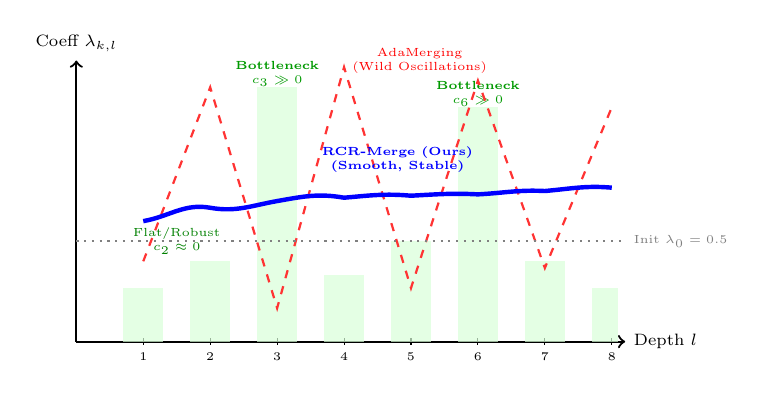
\begin{tikzpicture}[scale=0.85, every node/.style={scale=0.85}]
    % Grid and axes
    \draw[->, thick] (0,0) -- (8.2,0) node[right, font=\scriptsize] {Depth $l$};
    \draw[->, thick] (0,0) -- (0,4.2) node[above, font=\scriptsize] {Coeff $\lambda_{k, l}$};
    
    % X-axis ticks (layers)
    \foreach \x in {1, 2, 3, 4, 5, 6, 7, 8} {
        \draw (\x, 0.05) -- (\x, -0.05) node[below, font=\tiny] {\x};
    }
    
    % Draw Fisher Curvature Barriers (shaded green rectangles)
    \fill[green!15, opacity=0.7] (0.7,0) rectangle (1.3,0.8);
    \fill[green!15, opacity=0.7] (1.7,0) rectangle (2.3,1.2);
    \fill[green!15, opacity=0.7] (2.7,0) rectangle (3.3,3.8); % Bottleneck Layer 3
    \fill[green!15, opacity=0.7] (3.7,0) rectangle (4.3,1.0);
    \fill[green!15, opacity=0.7] (4.7,0) rectangle (5.3,1.5);
    \fill[green!15, opacity=0.7] (5.7,0) rectangle (6.3,3.5); % Bottleneck Layer 6
    \fill[green!15, opacity=0.7] (6.7,0) rectangle (7.3,1.2);
    \fill[green!15, opacity=0.7] (7.7,0) rectangle (8.1,0.8);
    
    % Labels for Curvature Barriers
    \node[green!60!black, font=\tiny\bfseries, align=center] at (3,4.0) {Bottleneck\\$c_3 \gg 0$};
    \node[green!60!black, font=\tiny\bfseries, align=center] at (6,3.7) {Bottleneck\\$c_6 \gg 0$};
    \node[green!50!black, font=\tiny, align=center] at (1.5,1.5) {Flat/Robust\\$c_2 \approx 0$};
    
    % Draw Unconstrained AdaMerging Trajectory (wild red zig-zag)
    \draw[red!80, thick, dashed, mark=*] (1, 1.2) -- (2, 3.8) -- (3, 0.5) -- (4, 4.1) -- (5, 0.8) -- (6, 3.9) -- (7, 1.1) -- (8, 3.5);
    \node[red, font=\tiny, align=center, right] at (4,4.2) {AdaMerging\\(Wild Oscillations)};
    
    % Draw RCR-Merge Trajectory (smooth coordinated blue curve)
    \draw[blue, ultra thick, mark=*] (1, 1.8) to[out=10, in=170] (2, 2.0) to[out=-10, in=190] (3, 2.1) to[out=10, in=170] (4, 2.15) to[out=5, in=175] (5, 2.18) to[out=3, in=177] (6, 2.2) to[out=3, in=177] (7, 2.25) to[out=5, in=175] (8, 2.3);
    \node[blue, font=\tiny\bfseries, align=center, above] at (4.8,2.4) {RCR-Merge (Ours)\\(Smooth, Stable)};
    
    % Draw baseline / initialization line (0.5)
    \draw[gray, dotted, thick] (0, 1.5) -- (8.2, 1.5) node[right, font=\tiny] {Init $\lambda_0 = 0.5$};
    
  \end{tikzpicture}
  \caption{Schematic concept diagram of the \textbf{Overfitting-Optimizer Paradox} and the stabilizing action of \textbf{RCR-Merge}. Unconstrained AdaMerging (dashed red) fits local transductive noise by generating high-frequency spatial oscillations across network depth. RCR-Merge (solid blue) weights spatial Total Variation by pre-trained base model curvatures $c_l$ (shaded green), establishing analytical coordinate barriers that block wild jumps in sensitive bottlenecks while permitting smooth, coordinated adaptation in robust layers.}
  \label{fig:schematic}
\end{figure}

\textbf{Summary of Contributions:}
\begin{itemize}
    \item We formulate and define the \textbf{Overfitting-Optimizer Paradox} in adaptive model merging, demonstrating both theoretically and empirically how unconstrained test-time entropy minimization under local stream bias collapses internal model representations.
    \item We introduce \textbf{RCR-Merge}, a novel second-order geometric framework that regularizes the spatial total variation of layer-wise merging coefficients by scaling adjacent-layer penalties with the trace of the base model's diagonal Fisher Information Matrix.
    \item We prove formal theoretical guarantees (Lemma~\ref{lem:coordinate_barrier} and Theorem~\ref{thm:representation_drift}) showing that our Riemannian curvature-weighted regularizer acts as an analytical barrier protecting representation integrity in highly sensitive layers.
    \item We conduct a rigorous 30-seed simulation study on the Coupled Model II Landscape emulator. RCR-Merge resolves the overfitting collapse, outperforming the static Uniform Baseline by \textbf{+3.06\% absolute}, unconstrained AdaMerging by \textbf{+10.33\% absolute}, and standard flat TV regularization by \textbf{+5.01\% absolute}, while demonstrating unparalleled stability and variance reduction.
\end{itemize}